\documentclass[tikz, border=25pt]{standalone}
\usepackage{xcolor}
\usepackage{helvet}
\renewcommand{\familydefault}{\sfdefault}
\usepackage{amsmath}
\usetikzlibrary{shapes.geometric, arrows.meta, positioning, fit, backgrounds, calc}

% Colors for Calibration
\definecolor{calbg}{HTML}{D9E8FD}
\definecolor{calborder}{HTML}{3B82F6}
\definecolor{calarrow}{HTML}{2563EB}

% Colors for Optimization
\definecolor{optbg}{HTML}{D1FAE5}
\definecolor{optborder}{HTML}{10B981}
\definecolor{optarrow}{HTML}{059669}

\definecolor{textcolor}{HTML}{0F172A}
\definecolor{containerbg}{HTML}{F8FAFC}
\definecolor{containerborder}{HTML}{CBD5E1}

\hyphenpenalty=10000
\exhyphenpenalty=10000

\tikzset{
  calbox/.style={
    draw=calborder,
    fill=calbg,
    line width=1.8pt,
    rounded corners=12pt,
    align=center,
    text=textcolor,
    font=\sffamily\bfseries\Large,
    inner sep=12pt,
    text width=12cm,
    minimum height=1.4cm
  },
  optbox/.style={
    draw=optborder,
    fill=optbg,
    line width=1.8pt,
    rounded corners=12pt,
    align=center,
    text=textcolor,
    font=\sffamily\bfseries\Large,
    inner sep=12pt,
    text width=12cm,
    minimum height=1.4cm
  },
  arrowc/.style={
    -{Stealth[length=14pt, width=11pt]},
    line width=3.5pt,
    color=calarrow,
    shorten >= 5pt,
    shorten <= 5pt
  },
  arrowo/.style={
    -{Stealth[length=14pt, width=11pt]},
    line width=3.5pt,
    color=optarrow,
    shorten >= 5pt,
    shorten <= 5pt
  },
  arrowtrans/.style={
    -{Stealth[length=16pt, width=13pt]},
    line width=4.5pt,
    color=textcolor,
    shorten >= 5pt,
    shorten <= 5pt
  },
  container/.style={
    draw=containerborder,
    fill=containerbg,
    line width=2.5pt,
    rounded corners=20pt,
    inner sep=20pt
  }
}

\begin{document}
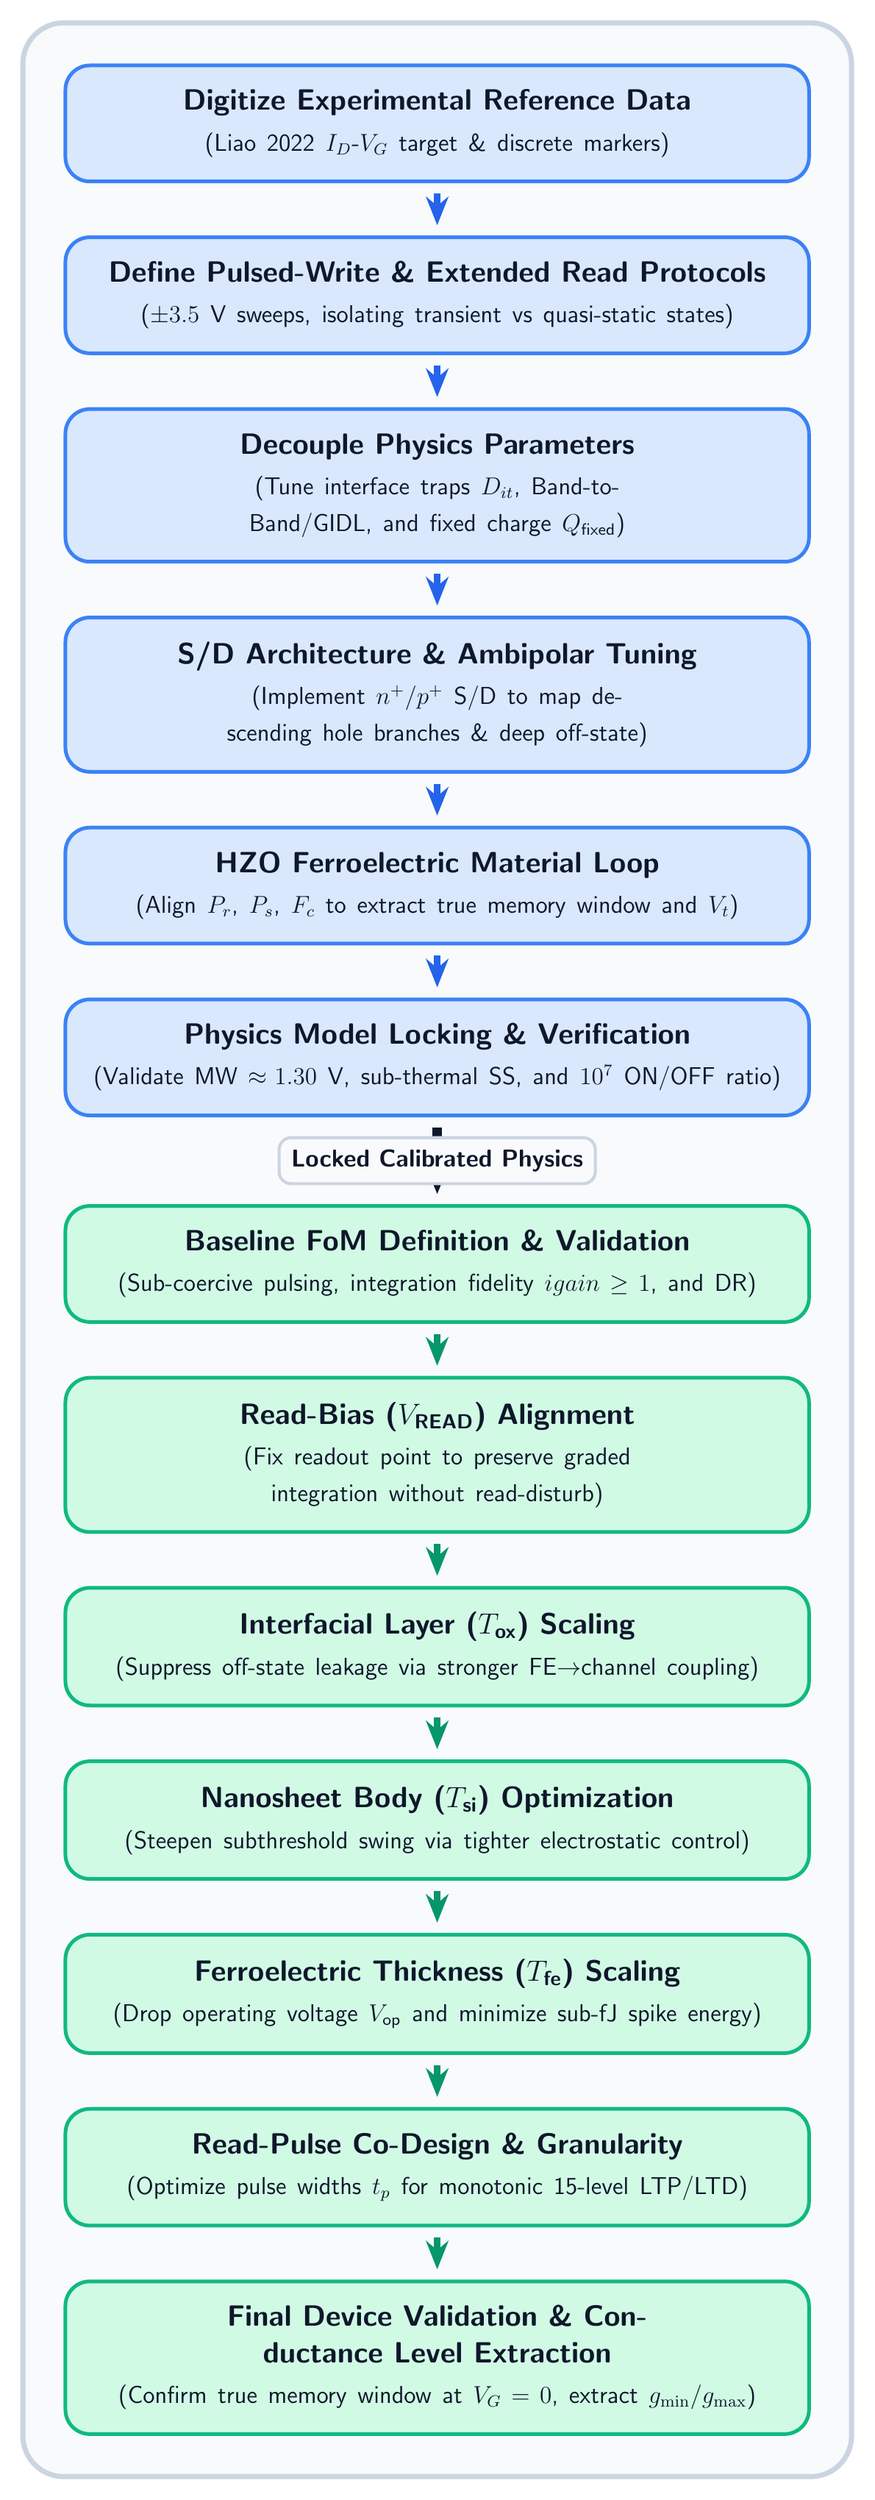
\begin{tikzpicture}[node distance=0.9cm]

  % ==================== CALIBRATION ====================
  \node (c1) [calbox] {Digitize Experimental Reference Data\\[2pt]{\large\normalfont(Liao 2022 $I_D\text{-}V_G$ target \& discrete markers)}};
  
  \node (c2) [calbox, below=of c1] {Define Pulsed-Write \& Extended Read Protocols\\[2pt]{\large\normalfont($\pm3.5$ V sweeps, isolating transient vs quasi-static states)}};
  
  \node (c3) [calbox, below=of c2] {Decouple Physics Parameters\\[2pt]{\large\normalfont(Tune interface traps $D_{it}$, Band-to-Band/GIDL, and fixed charge $Q_{\text{fixed}}$)}};
  
  \node (c4) [calbox, below=of c3] {S/D Architecture \& Ambipolar Tuning\\[2pt]{\large\normalfont(Implement $n^+/p^+$ S/D to map descending hole branches \& deep off-state)}};
  
  \node (c5) [calbox, below=of c4] {HZO Ferroelectric Material Loop\\[2pt]{\large\normalfont(Align $P_r$, $P_s$, $F_c$ to extract true memory window and $V_t$)}};
  
  \node (c6) [calbox, below=of c5] {Physics Model Locking \& Verification\\[2pt]{\large\normalfont(Validate MW $\approx 1.30$ V, sub-thermal SS, and $10^7$ ON/OFF ratio)}};

  % ==================== OPTIMIZATION ====================
  \node (o1) [optbox, below=1.5cm of c6] {Baseline FoM Definition \& Validation\\[2pt]{\large\normalfont(Sub-coercive pulsing, integration fidelity $igain \geq 1$, and DR)}};
  
  \node (o2) [optbox, below=of o1] {Read-Bias ($V_{\text{READ}}$) Alignment\\[2pt]{\large\normalfont(Fix readout point to preserve graded integration without read-disturb)}};
  
  \node (o3) [optbox, below=of o2] {Interfacial Layer ($T_{\text{ox}}$) Scaling\\[2pt]{\large\normalfont(Suppress off-state leakage via stronger FE$\rightarrow$channel coupling)}};
  
  \node (o4) [optbox, below=of o3] {Nanosheet Body ($T_{\text{si}}$) Optimization\\[2pt]{\large\normalfont(Steepen subthreshold swing via tighter electrostatic control)}};
  
  \node (o5) [optbox, below=of o4] {Ferroelectric Thickness ($T_{\text{fe}}$) Scaling\\[2pt]{\large\normalfont(Drop operating voltage $V_{\text{op}}$ and minimize sub-fJ spike energy)}};
  
  \node (o6) [optbox, below=of o5] {Read-Pulse Co-Design \& Granularity\\[2pt]{\large\normalfont(Optimize pulse widths $t_p$ for monotonic 15-level LTP/LTD)}};
  
  \node (o7) [optbox, below=of o6] {Final Device Validation \& Conductance Level Extraction\\[2pt]{\large\normalfont(Confirm true memory window at $V_G=0$, extract $g_{\min}/g_{\max}$)}};

  % Background container
  \begin{scope}[on background layer]
    \node (fitbox) [container, fit=(c1) (c6) (o1) (o7)] {};
  \end{scope}

  % Connectors Calibration
  \draw [arrowc] (c1) -- (c2);
  \draw [arrowc] (c2) -- (c3);
  \draw [arrowc] (c3) -- (c4);
  \draw [arrowc] (c4) -- (c5);
  \draw [arrowc] (c5) -- (c6);

  % Transition Connector
  \draw [arrowtrans] (c6) -- (o1) node[midway, fill=containerbg, inner sep=6pt, font=\sffamily\bfseries\large, text=textcolor, draw=containerborder, rounded corners=6pt, line width=1.5pt] {Locked Calibrated Physics};

  % Connectors Optimization
  \draw [arrowo] (o1) -- (o2);
  \draw [arrowo] (o2) -- (o3);
  \draw [arrowo] (o3) -- (o4);
  \draw [arrowo] (o4) -- (o5);
  \draw [arrowo] (o5) -- (o6);
  \draw [arrowo] (o6) -- (o7);

\end{tikzpicture}
\end{document}
